\chapter{Introduction} \label{ch:Introduction} % (2 pages)

\section{Problem Statement} \label{sec:ProblemStatement}
In a production line, different work pieces have be checked in the beginning to make sure only work pieces which meet all requirements are further processed. Therefore a MPS testing station of the vendor Festo is used, which provides a set of sensors and work piece handling components / actuators (see Fig.\ref{fig:festostation}). The sensors and actuators of the station are connected to the GPIO Pins of the micro-controller of the \textit{Tiva Development Kit DK-TM4C129X}. This allows controlling the actuators (activation or deactivation) and reading sensor values.

\begin{figure}[H]
	\begin{center}
		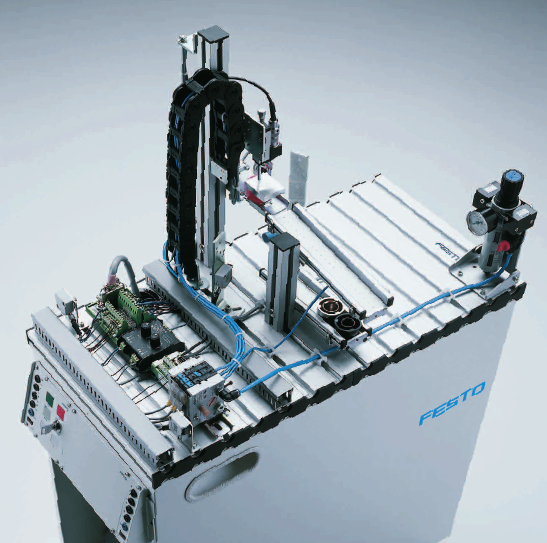
\includegraphics[scale=.50]{media/FestoStation.png} 	
		\caption{Festo Station}
		\label{fig:festostation}
	\end{center}
\end{figure}

The testing process is structured into the following steps:
\begin{enumerate}[noitemsep]
	\item Workpiece is placed onto a platform.
	\item Color and material is sensed with the related sensors in this position(see Fig. \ref{fig:festostationsensorsandejector} and Fig.\ref{fig:festostationcolorandmaterialsensor}).
	\item A safety light barrier is used to ensure that the hands of the operator of the station are not in the zone of the moving parts any more.
	\item The platform is moved up (see Fig.\ref{fig:festostationliftingmodule}).
	\item In the top position a height measurement is triggered (see Fig.\ref{fig:festostationheightmeasurement}).
	\item Based on the height measurement a work piece is accepted within certain thresholds or rejected if beyond.
	\item If the work piece is accepted the following steps are executed:
	\begin{enumerate}
		\item The ejector which is attached to the platform pushes the work piece onto a pneumatic slide (see Fig.\ref{fig:festostationsensorsandejector}). 
		\item The pneumatic slide is activated to transfer the work piece to the next station in the production process (see Fig.\ref{fig:festostationpneumaticslide}).
		\item The ejector is retracted.
		\item The platform is moved down.
	\end{enumerate} 
	\item If it is rejected the following steps are executed:
	\begin{enumerate}
		\item The platform is moved down.
		\item The ejector which is attached to the platform pushes the work piece onto a  slide which is not further automated.
		\item The ejector is retracted.
	\end{enumerate}
\end{enumerate}


\begin{figure} [H] 	
	\begin{center}
		\subfigure[Festo Station Height Measurement]{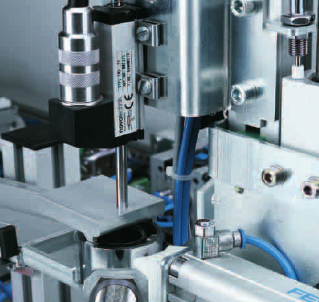
\includegraphics[width=0.4\textwidth]{media/FestoStation_HeighMeasurement.png}
			\label{fig:festostationheightmeasurement}} 
		\hspace{0.05\textwidth}
		\subfigure[Festo Station Senors and Ejector]{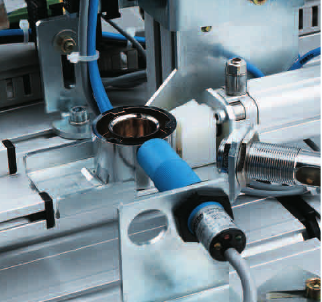
\includegraphics[width=0.4\textwidth]{media/FestoStation_SensorsAndEjector.png}
			\label{fig:festostationsensorsandejector}} 
		\caption{Festo Station Detail}
		\label{fig:festostationdetail}
	\end{center}
\end{figure} 

\begin{figure} [H] 	
	\begin{center}
		\subfigure[Festo Color and Material Sensor]{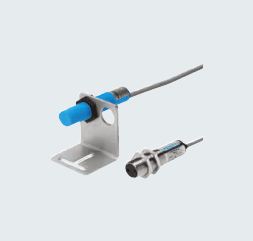
\includegraphics[width=0.25\textwidth]{media/FestoStation_ColorAndMaterialSensor.png}
			\label{fig:festostationcolorandmaterialsensor}} 
		\hspace{0.05\textwidth}
		\subfigure[Festo Lifting Module]{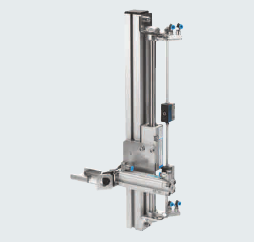
\includegraphics[width=0.25\textwidth]{media/FestoStation_LiftingModule.png}
			\label{fig:festostationliftingmodule}} 
		\hspace{0.05\textwidth}
		\subfigure[Festo Pneumatic Slide]{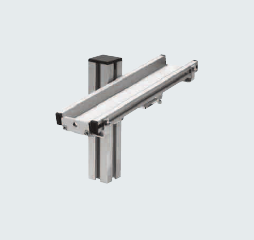
\includegraphics[width=0.25\textwidth]{media/FestoStation_PneumaticSlide.png}
			\label{fig:festostationpneumaticslide}} 
		\caption{Festo Modules Detail}
		\label{fig:festomodulesdetail}
	\end{center}
\end{figure} 

\section{Requirements}
The task was to fully automate the testing process by implementing a test program which runs on the micro-controller and operates based on the sensor values as an input and controls the actuators in a real time manner. The Task was spilt up into two sections:
Firstly a device driver should be written to allow a high level access to the GPIO ports, encapsulated in meaningful methods. The device driver should provide methods for each of the tasks (and subtasks) mentioned in section \ref{sec:ProblemStatement}. A special requirement was also the conversion of the analogue height measurement signal to a meaningful digital value.
Secondly an application program should be written which controls the execution of the testing process, allows the user to start, stop and configure it and display relevant information on the touch screen of the Tiva development board. This included methods for the calibration of the height measurement, the setting of threshold values and keeping track of all processed work pieces. Additionally the calendar time should be displayed and a throughput should be calculated.

\section{Contributions}
The display logic and the interaction with the main program was developed by Julian Daberkow. The device driver was developed by Timo Michalski and Hendrik Oestreich and integrated into the main program. They also developed the state machine which controls the execution of the testing process. The overall integration of all components including the communication between the different tasks was done by Julian Daberkow and Timo Michalski. 





